
\label{sec:equivalence}
\twoSortedRBAC{} \cite{two-sorted-rbac} is an interesting extension of Role Based Access Control which breaks the duality of roles (users and permissions perspectives) into proper roles ($\properRole$) as group of users and demarcations ($\demarcation$) as groups of permissions. User inheritance is maintained with proper role hierarchy ($\properRoleHierarchy$) and permission inheritance is maintained with demarcation hierarchy ($\demarcationHierarchy$). The connection between proper roles and demarcation is maintained by the grant relation ($G$) which enumerates (proper role, demarcation) pairs. For example, for proper roles and demarcations given in Figure \ref{fig:two-sorted-rbac-example}, G includes following tuples - \{(manager, red), (employee, amber)\}. Note that \twoSortedRBAC{} \cite{two-sorted-rbac} also includes negative roles and demarcations which we do not consider here.



\twoSortedRBAC{} is compelling in many ways. It introduces a higher administrative level (through grant relation) for access management. User-role assignment ($UR^+ \subseteq U \times \properRole$) and demarcation-permission assignment ($PD^+ \subseteq P \times \demarcation$), along with administration of grant relation can be carried out more independently and distributively. Moreover, the authors shows that, \twoSortedRBAC{} enables many-to-many administrative mutations which leads to organizational scalability.  In many-to-many mutation, by granting a (proper role, demarcation) pair, all users in the proper role get all  permissions in the demarcation which, as the authors shows cannot be achieved by standard RBAC \cite{nist-rbac}.


  \begin{figure}
 	\centering
 	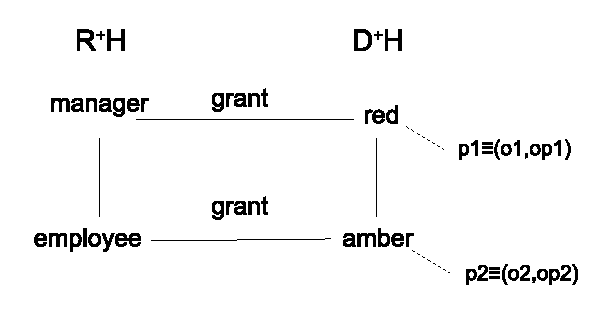
\includegraphics[width=.7\textwidth]{ABAC16/two-sorted-rbac-example}
 	\caption{An example of Two-sorted-RBAC}
 	\label{fig:two-sorted-rbac-example}
 \end{figure} 

 

The benefits of \twoSortedRBAC{} can also be realized through \eapABAC{}. For example, user to $\uLabel{}$ value assignments, object to $\oLabel{}$ value assignments and authorization policies are analogous to $\properRoleHierarchy$, $\demarcationHierarchy$ and grant relation in \twoSortedRBAC{} and  can also be carried out independently. On the other hand, many-to-many administrative mutation can also be achieved. For example, the \eapABAC{} policy, $\Policy_{op1}\equiv \{(manager, (red,op1))\}$ in Figure \ref{fig:two-sorted-rbac-to-labac-example},  enables every   $manager$ to perform operation $op1$ on every object labeled with  $(red,op1)$. 

 \begin{figure}
 	\centering
 	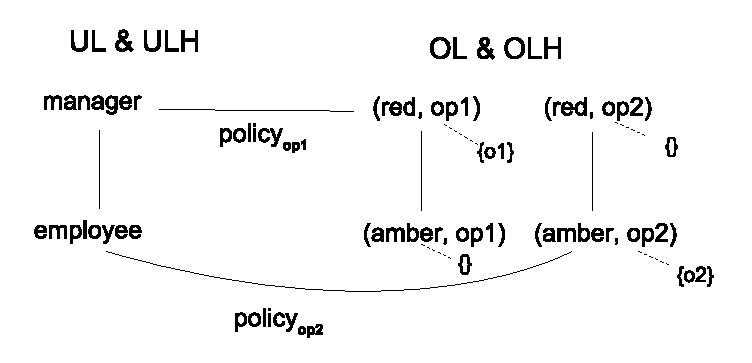
\includegraphics[width=.7\textwidth]{ABAC16/two-sorted-rbac-to-labac-example}
 	\caption{An example of \twoSortedRBAC{} configured in \eapABAC{}}
 	\label{fig:two-sorted-rbac-to-labac-example}
 \end{figure}
 


 \begin{table}
	\centering
	\caption{ \twoSortedRBAC{} in \hlabac} %\vspace*{3pt}
	\label{tab:two-sorted-rbac-in-labac-table}
	\begin{tabular}{|l|}						
		\hline					
		\multicolumn{1}{|c|}{\underline{\textit{I. \twoSortedRBAC{} components }}}\\	\\			 
		 -  $S, OBS, OPS$, $\roles, \RH$, $\demarcation, \DeH$,   (users, objects,   operations, proper roles, \\ \hfill role hierarchy, demarcation  and demarcation hierarchy respectively). \\
		 -  $PRMS = {(OBS \times OPS)}$, the set of permissions  \\		 
		 -  $\SR \subseteq S \times \roles$  \\
		 -  $\PD \subseteq PRMS \times \demarcation$ \\	 
		 - $G \subseteq \roles \times \demarcation$\\
		\\ \multicolumn{1}{|c|}{\underline{\textit{II. Construction in \hlabac{}}}} \\ \\
		 	-  $U = S, O = OBS, A = OPS $ \\ 
		 	- $UL=\roles, ULH=\RH$\\		  
		 	- $ OL = \demarcation \times OPS$\\
		 	- $OLH= \{ ((d_i, op_i), (d_j, op_j)) | d_i  \succeq d_j \land op_i = op_j\}$\\
		 	-  $\uLabel(u) = \{ r | (s,r) \in \SR \}$ \\		 	
		 	-  $ \oLabel(o) = \{ (d,op) | ((o,op),d) \in PD \}$\\		 	 	
		 	-  $\policy_{op_i} = \{ (r_i, (d_j,op_j) ) |  (r_i,d_i) \in G \land$ $((o,op_i),d_i)  \in \PD \} $ \\
		 \hline	
	\end{tabular}	

	
\end{table}

 
 \eapABAC{} is similar to \twoSortedRBAC{} in spirit. While \twoSortedRBAC{} is more role oriented, \eapABAC{} is attribute oriented. In the rest of this section, we show equivalence of \eapABAC{} and \twoSortedRBAC{} with respect to their theoretical  expressive power. In order to establish the equivalence, we show that any instance of \twoSortedRBAC{} can be expressed in \eapABAC{} and vice-versa.

 
 
Figure  \ref{fig:two-sorted-rbac-to-labac-example} is an example showing configuration of a \twoSortedRBAC{} instance (given in Figure \ref{fig:two-sorted-rbac-example}) in \eapABAC{}. In Figure  \ref{fig:two-sorted-rbac-to-labac-example}, user-label values and its hierarchy directly corresponds to roles and role hierarchy in Figure \ref{fig:two-sorted-rbac-example}. On the other hand, object-label values correspond to Cartesian product of $\demarcation$ and $OPS$.   An object-label value $(d_i, op)$ dominates another object-label value $(d_j, op)$, if demarcation $d_i$ dominates demarcation $d_j$. For example, for demarcations \{$red$, $amber$\} and operations $\{op1,op2\}$ (of Figure \ref{fig:two-sorted-rbac-example}), four object-label values have been defined where $(red,op1)$ dominates $(amber,op1)$ because $red$ dominates $amber$.  For an object-label value $(d,op)$, we assign $(d,op)$ to the object $o$ to if $(o,op)$ is a permission in demarcation $d$. For example, object $o1$ is assigned the value $(red,op1)$ because $(o1,op1)$ is  a permission in demarcation $red$.  On the other hand, user-label values assigned to a user corresponds to his assigned proper roles. Finally, having assigned object-label and user-label values, for each grant relation $(r,d) \in G$,  we specify authorization policy $Policy_{op} \equiv \{(r,(d,op))\}$ so that object labeled with $(d,op)$ are accessed by users with role $r$ for operation $op$. For example, for the grant relation $(manager,red)$ in Figure \ref{fig:two-sorted-rbac-example}, we create a policy $Policy_{op1} \equiv \{(manager, (red,op1))\}$. We do not create  policy $Policy_{op2} \equiv \{(manager, (red,op2))\}$ because there is no permission defined with operation $op2$ in demarcation $red$. Table \ref{tab:two-sorted-rbac-in-labac-table}  shows this configuration formally.
 

 
 %  \begin{figure}[!htbp]
 	\centering
 	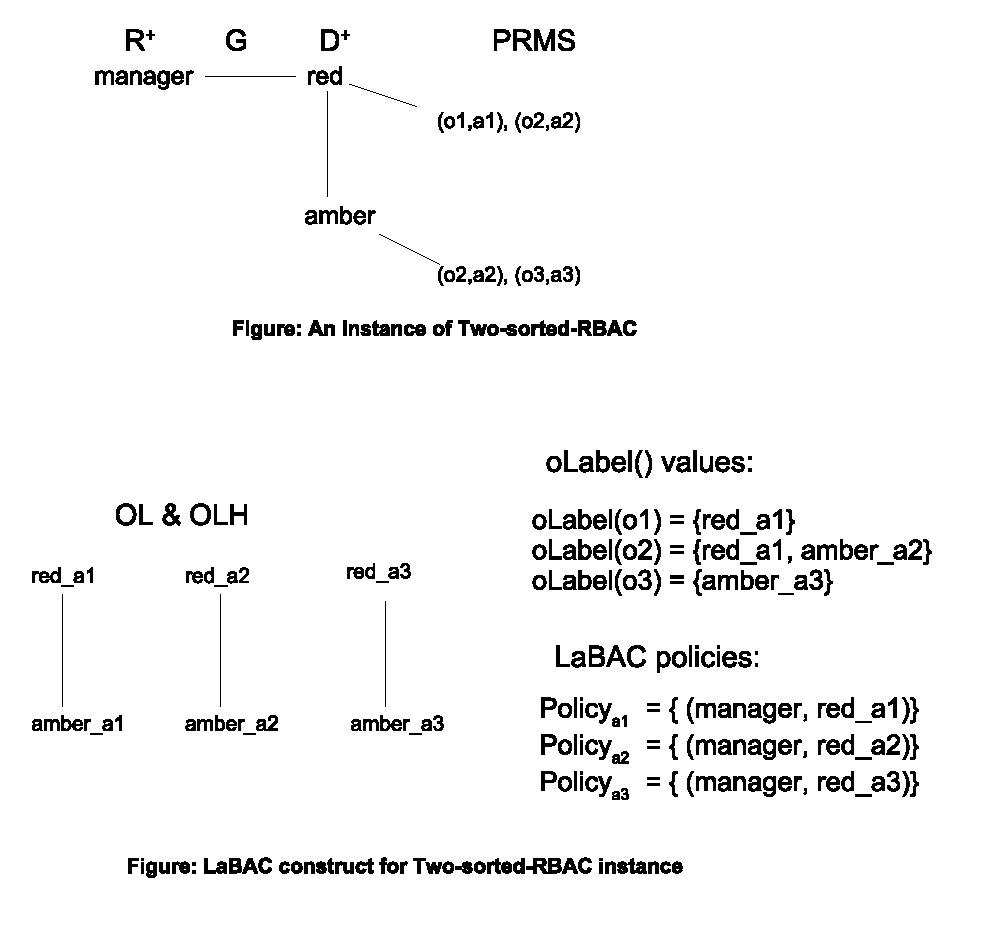
\includegraphics[width=.6\textwidth]{two-sorted-labac-example-diagram}
 	\caption{A $RBAC_1$ instance of role and perms.}
 	\label{fig:two-sorted-labac-example-diagram}
 \end{figure}
 
 \begin{table}
	\centering
	\caption{ \hlabac{} in \twoSortedRBAC{} } %\vspace*{3pt}
	\label{tab:labac-in-two-sorted-rbac-table}
	\begin{tabular}{|l|}						
		\hline					
			\multicolumn{1}{|c|}{\underline{\textit{I. \hlabac{} components}}} \\
			-  $U, O,  A$ (set of users, objects and actions resp.) \\ 
%			- $UL, OL, ULH,  OLH$ (uLabel and oLabel values, \\ \hfill uLabel and oLabel value hierarchy  resp.) \\		  
%			-  $\uLabel()$, user to user-label value assignment relation \\		 	
%			-  $\oLabel()$, object to object-label value assignment relation \\
%			-  $\policy_{a}$, LaBAC authorization policies for $a \in A$\\\\
			- $UL, OL, ULH,  OLH$ (uLabel values, oLabel values, \\ \hfill uLabel and oLabel value hierarchy  resp.) \\		  
			-  $\uLabel: U \to 2^{UL}$, $\oLabel: O \to 2^{OL}$ \\
			-  $\Policy_{a}$, authorization policy for action $a \in A$\\
		
		\\ \multicolumn{1}{|c|}{\underline{\textit{II. Construction in \twoSortedRBAC}}}\\	
		- $S=U, OBS=O, OPS=A$\\			 
		 - $\properRole = UL$, $\properRoleHierarchy = ULH$ \\ 
 		 - $\demarcation = OL$, $\demarcationHierarchy = \{\}$ \\ 
 		 - $\SR = \{ (u,r) | r \in uLabel(u)\}$\\
 		 - $\PD = \{ ((o_i, a_i), ol) | \exists (ul,ol) \in \policy_{a_i} \land$ \\ \hfill $ol' \in oLabel(o_i) \land ol \odominate ol'\}$ \\
 		 - $G = \{ (ul,ol) | (ul,ol) \in \policy_a  \}$\\
		\hline	
	\end{tabular}	

	
\end{table}

 
 
 
 Configuration of \hlabac{} in \twoSortedRBAC{} is given in Table \ref{tab:labac-in-two-sorted-rbac-table}. Segment I represents elements of \eapABAC{} model and Segment II shows the configuration of \twoSortedRBAC{}.  In the configuration, user-label values and its hierarchy are used as proper roles and proper role hierarchy. Object-label values are used as names for demarcations. For an object-label value $ol\in OL$, let $O_{ol}$ be the objects labeled with $ol$. For each policy $policy_{op} \equiv \{(ul, ol)\}$ in \eapABAC{}, we create a grant relation $(ul,ol)$ in \twoSortedRBAC{}. Further, assign permission (o,op) in demarcation named $ol$ for $o \in O_{op}$. Note that \twoSortedRBAC{} does not distinguish between users and sessions as we do in \eapABAC{}. For this reason, we omit \eapABAC{} sessions while showing equivalence with \twoSortedRBAC{}.
 
 
 

  
  Here we use \hlabac{} to configure \twoSortedRBAC{} for convenience. In fact,  \clabac{} is the minimalistic model that is equivalent to \twoSortedRBAC{}. In Figure \ref{fig:expressiveness-spectrum}, we show summary of expressive power of different \eapABAC{} models. The dashed box represents the minimalistic \eapABAC{} model required to configure other models and solid box represents the \eapABAC{} model that we use for our convenience. 

%We acknowledge the more formal  approach of \textit{state matching reduction} or simply \textit{reduction} \cite{tripli} for establishing equivalence between access control models. For simplicity and absence of state transition functions (administrative models) for some models discussed here, we adopt a simplified and conventional approach for the establishment of  equivalence.

The construction of Tables \ref{tab:two-sorted-rbac-in-labac-table} and \ref{tab:labac-in-two-sorted-rbac-table} and other constructions given in the rest of this paper can be cast in the formal approach of \cite{tripli}. So, these models are equivalent in the sense of state-matching reduction. 

   \begin{figure}
 	\centering
 	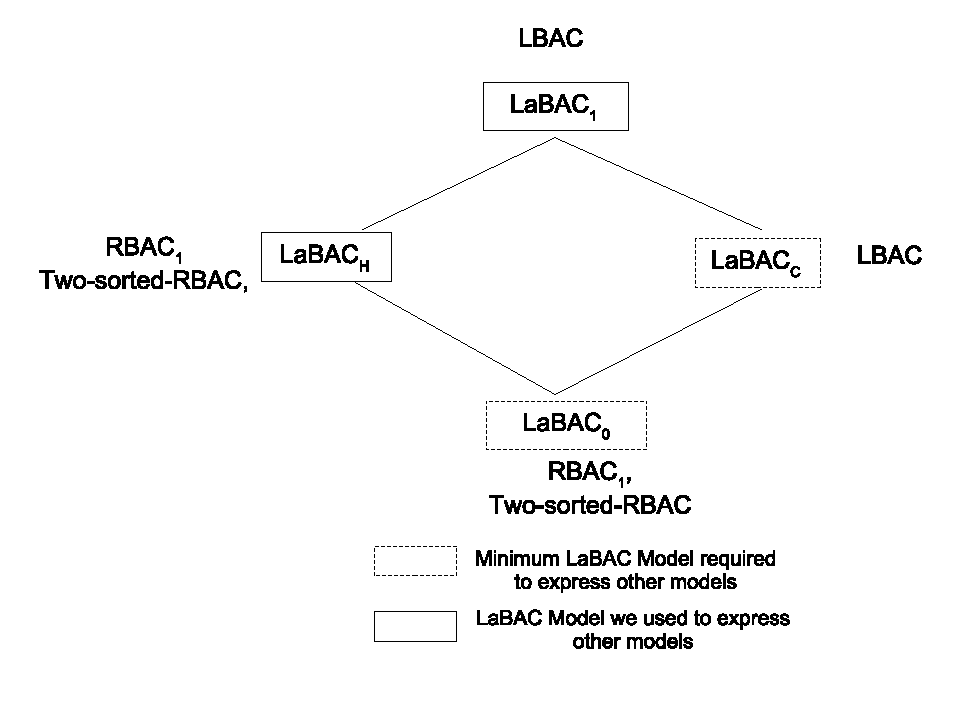
\includegraphics[width=.8\textwidth]{ABAC16/expressiveness-spectrum}
 	\caption{Expressiveness of LaBAC models}
 	\label{fig:expressiveness-spectrum}
 \end{figure}
 
